% !TEX program = xelatex
% Build: `tectonic main.tex` from this folder (XeTeX engine; on Overleaf choose XeLaTeX).
% Figures: `PYTHONPATH=src .venv/bin/python paper/make_figures.py` from the repo root.
% Tables:  `.venv/bin/python paper/make_tables.py` from the repo root (numbers come from runs/).
\documentclass[11pt,letterpaper]{article}

\usepackage[letterpaper,top=1in,bottom=1in,left=1.05in,right=1.05in,headheight=14pt]{geometry}
\renewcommand{\rmdefault}{Cochineal-TLF}
\usepackage[cochineal,vvarbb]{newtxmath}
\usepackage[no-math]{fontspec}
\setmainfont{Cochineal}[
  Extension      = .otf,
  UprightFont    = *-Roman,
  ItalicFont     = *-Italic,
  BoldFont       = *-Bold,
  BoldItalicFont = *-BoldItalic,
  Numbers        = {Lining,Proportional},
  Ligatures      = NoCommon,
  WordSpace      = {1.3,1.3,0.3}]
\setmonofont{Inconsolatazi4}[
  Extension   = .otf,
  UprightFont = *-Regular,
  BoldFont    = *-Bold,
  Scale       = MatchLowercase]

\usepackage[protrusion=true,expansion=false]{microtype}
\usepackage{amsmath}
\usepackage{graphicx}
\usepackage{booktabs,tabularx,array}
\usepackage[font=small,labelfont=bf,labelsep=period,skip=5pt]{caption}
\usepackage{enumitem}
\usepackage{xcolor}
\usepackage[round,authoryear]{natbib}
\renewcommand{\bibfont}{\small\raggedright}
\setlength{\bibsep}{5pt}
\usepackage{fancyhdr}
\usepackage{hyperref}
\usepackage[numbered]{bookmark}

\definecolor{linkblue}{HTML}{1F3A68}
\hypersetup{
  colorlinks = true,
  linkcolor  = linkblue,
  citecolor  = linkblue,
  urlcolor   = linkblue,
  pdftitle   = {Small Updates Break First: A Pre-Registered Study of Fine-Tuning Gains Under MLX and GGUF Quantization},
  pdfauthor  = {Jayesh Suryavanshi},
  pdfsubject = {Draft of 29 September 2026},
  pdfkeywords = {quantization, LoRA, fine-tuning, MLX, GGUF, pre-registration}}

\linespread{1.07}
\exhyphenpenalty=10000
\hyphenation{LoRA LoRAs OLMo}
\renewcommand{\topfraction}{0.88}
\renewcommand{\bottomfraction}{0.6}
\renewcommand{\textfraction}{0.08}
\renewcommand{\floatpagefraction}{0.8}
\setcounter{topnumber}{3}
\setcounter{bottomnumber}{2}
\setcounter{totalnumber}{5}
\setlength{\parskip}{0pt}
\setlist{itemsep=3pt,topsep=4pt,parsep=0pt}
\renewcommand{\arraystretch}{1.12}
\newcolumntype{L}{>{\raggedright\arraybackslash}X}
\newcommand*{\tablerows}[1]{\csname @@input\endcsname #1 }

\pagestyle{fancy}
\fancyhf{}
\fancyhead[L]{\small\itshape Small updates break first}
\fancyhead[R]{\small\itshape Draft, 29 September 2026}
\fancyfoot[C]{\small\thepage}
\renewcommand{\headrulewidth}{0.4pt}
\fancypagestyle{plain}{\fancyhf{}\fancyfoot[C]{\small\thepage}\renewcommand{\headrulewidth}{0pt}}

\begin{document}

\thispagestyle{plain}
\begin{center}
  {\LARGE\bfseries Small Updates Break First\par}
  \vspace{6pt}
  {\Large A Pre-Registered Study of Fine-Tuning Gains\\ Under MLX and GGUF Quantization\par}
  \vspace{14pt}
  {\large Jayesh Suryavanshi\par}
  \vspace{2pt}
  {\small\href{mailto:jayeshksuryavanshi@gmail.com}{\texttt{jayeshksuryavanshi@gmail.com}}\par}
  \vspace{8pt}
  {\small\itshape Draft of 29 September 2026. Not peer reviewed.\par}
\end{center}
\vspace{4pt}

\begin{abstract}
\noindent
Small language models are routinely fine-tuned and then shipped at 3 to 6 bits per weight, as MLX affine or GGUF k-quant files, on the assumption that the fine-tuning gain survives. We tested that assumption in four pre-registered rounds on a single laptop. We fine-tuned Qwen3 at 0.6B, 1.7B and 4B parameters and OLMo-2 1B with LoRA (and, on Qwen3-0.6B, full fine-tuning) on banking77 intent classification and MASSIVE slot annotation, and evaluated every model on its full test set at bf16 and up to ten quantized formats. The fine-tunes that lost the most were the gentle ones, trained at low learning rates with small updates. In all 10 pre-registered tests of this comparison, a LoRA trained at learning rate $10^{-4}$ kept more of its gain at MLX~3-bit and GGUF~Q3\_K\_M than the same LoRA at $10^{-5}$. In an exploratory count across seven settings, the gentler LoRA was the more accurate model at bf16, yet kept less of its accuracy at each of the five formats compared, from MLX~4-bit and Q4\_K\_M down to Q2\_K. Weight-space measurements are consistent with this: quantization usually preserves the component of the update along its own direction, but adds rounding noise that can be several times larger than the update, so a small update either drowns in the noise or is rounded away. A three-parameter model built from these measurements and the base model's own quantization damage predicted gain retention without evaluating the quantized fine-tune, with mean absolute error 0.059 and 0.084 on two pre-registered held-out tests, lower than bit-width and base-damage baselines (in the second test, its interval overlaps the base-damage baseline's). Its first version missed its pre-registered accuracy bar, and the current version misses on our 4B fine-tunes. In exploratory analyses, the share of items a confidence gate accepts fell faster than accuracy at 3 bits and below; the one pre-registered test of this, at 4 bits, was not supported.
\end{abstract}

\section{Introduction}
\label{sec:intro}

Fine-tuning a small open model and quantizing it for local inference has become a routine way to ship a task-specific language model. The artifact is usually an MLX model for Apple silicon \citep{mlx2023} or a GGUF file for llama.cpp \citep{llamacpp} and the tools built on it, at 3 to 6 bits per weight. Quantization methods are mostly evaluated on base models, with perplexity and broad benchmarks, and a fine-tune is assumed to keep what it learned. There are signs that it may not: merging a LoRA adapter into a native 4-bit checkpoint and writing it back through the quantizer can delete the adaptation \citep{li2026scaleqlora}.

This paper asks a narrower question with controlled evidence. When a fine-tuned model is quantized with the formats practitioners use, how much of the fine-tuning gain survives, which fine-tunes lose it, and can the loss be predicted from the weights before quantizing? We answered it in four rounds of experiments, each pre-registered and hashed before its confirmatory runs, on one Apple M1 Pro laptop with 16 GB of memory. The study covers Qwen3 at 0.6B, 1.7B and 4B parameters \citep{qwen3} and OLMo-2 1B \citep{olmo2}; banking77 intent classification \citep{casanueva2020banking77} and MASSIVE slot annotation \citep{fitzgerald2023massive}; LoRA \citep{hu2022lora} at learning rates from $3\times10^{-6}$ to $3\times10^{-4}$, and full fine-tuning on Qwen3-0.6B; and MLX affine quantization from 8 to 2 bits and GGUF quantization from Q8\_0 to Q2\_K. Every model was evaluated on its complete test set in both engines. Our findings:

\begin{itemize}
\item \textbf{Small updates break first.} We call a LoRA trained at learning rate $10^{-5}$ gentle and one trained at $10^{-4}$ strong. In all 10 pre-registered tests of this comparison (five pairs of LoRAs: OLMo-2 1B on banking77 and Qwen3-0.6B on MASSIVE, each with two seeds, and Qwen3-4B on banking77, each pair tested at MLX~3-bit and GGUF~Q3\_K\_M), the strong LoRA kept more of its gain than the gentle one (Section~\ref{sec:replication}). In an exploratory count over seven settings, the gentle LoRA was the more accurate model at bf16 and still kept less of its accuracy at each of the five formats compared. Choosing a fine-tune by its bf16 score can pick the one that degrades most.
\item \textbf{Two ways to fail.} Quantization usually preserves the component of the update along its own direction: in 168 of 192 fine-tune and format pairs, at least 98\% of that projection survived. What it adds is rounding noise, often several times larger than the update. A small update either drowns in that noise or, when the fine-tuned and base weights fall into the same quantization bins, is rounded away (Sections~\ref{sec:mechanism} and~\ref{sec:mech-results}).
\item \textbf{A predictor, held to its own bar.} A three-parameter model built from those measurements and the base model's own quantization damage predicted gain retention without evaluating the quantized fine-tune, with mean absolute error 0.059 and 0.084 on two pre-registered held-out tests, below bit-width and base-damage baselines. Its first version missed its pre-registered bar; the first version would also have passed the two later tests, and the current version misses on our 4B fine-tunes (Section~\ref{sec:predictor}).
\item \textbf{Operating points can move first.} In exploratory analyses, at a confidence threshold fitted at full precision, the share of items a quantized model accepts often fell much faster than its accuracy. The one pre-registered test of this, at 4 bits, was not supported (Section~\ref{sec:drift}).
\item \textbf{A tool.} \texttt{ftquant check} computes the measurements from the weights alone, with numpy on a CPU (Section~\ref{sec:tool}).
\end{itemize}

Every pre-registered result is reported, including the hypotheses that were not supported and the criterion the first predictor failed. Five deviations from the pre-registered plans are listed in Appendix~\ref{app:deviations}.

\section{Related work}
\label{sec:related}

\paragraph{Post-training quantization.} LLM.int8() \citep{dettmers2022llmint8}, GPTQ \citep{frantar2023gptq} and AWQ \citep{lin2024awq} showed that large language models can be quantized to 8 and 4 bits with little loss on standard benchmarks. Local inference stacks mostly use simpler formats that need no calibration data: MLX's affine quantization, with a scale and a bias per group of weights \citep{mlx2023}, and llama.cpp's GGUF block formats, including the mixed-precision k-quants \citep{llamacpp}. We study these formats as a practitioner would use them, without importance matrices or calibration.

\paragraph{Fine-tuning meets quantization.} LoRA \citep{hu2022lora} trains a low-rank update that can be merged into the base weights, and QLoRA \citep{dettmers2023qlora} trains it on top of a 4-bit base. What happens when a merged model is quantized again has had less attention. \citet{li2026scaleqlora} show that on native 4-bit microscaling checkpoints (NVFP4, MXFP4), naively merging and re-quantizing deletes the adaptation, by up to 39 points, because against an already on-grid base the reconstruction optimum is the base itself; they avoid this by adapting only the per-block scales. In mlx-lm, fusing an adapter into a pre-quantized gpt-oss-20b gave a model with 0\% task success while the unfused adapter worked \citep{mlxlm1172}. A proposed fix, closed without merging, attributed this to LoRA deltas of at most about $2.2\times10^{-3}$ (mean $2.4\times10^{-4}$) against a 4-bit quantization step of about $8.4\times10^{-2}$ \citep{mlxlm1564}, although the reporter saw the same failure with a dequantized fp16 fuse. Our rounded-away failure mode (Section~\ref{sec:mechanism}) rests on the same arithmetic, in the more common pipeline of fusing in bf16 and quantizing afterwards. We measure how often it occurs, identify a second, noise-dominated mode, and relate both to the size of the update.

\paragraph{Predicting what quantization breaks.} \citet{wu2026decisions} model how decision margins shrink under quantization and predict flip rates with a median error of 1.0 percentage point across 1,154 combinations of 16 models, quantization settings, bit widths and decision types. Their approach works from margins measured on task inputs; ours uses only the weights and a one-time measurement of the base model. The round-1 plan named their margin model as a future baseline; the round-2 plan replaced it with two simpler baselines, and a comparison remains open. \citet{zhu2026conformal} show that configuration shifts, including weight quantization, erode the coverage guarantees of conformal prediction. Our operating-point results (Section~\ref{sec:drift}) are a single-threshold counterpart.

\paragraph{Pre-registration.} Fixing hypotheses, analyses and decision rules before seeing the data separates confirmation from exploration \citep{nosek2018prereg}. It is still uncommon in machine learning evaluation. We hash each plan, log every deviation with a timestamp, and report the criteria our own predictor failed.

\section{Experimental setup}
\label{sec:setup}

\paragraph{Models and tasks.} Table~\ref{tab:bases} lists the base models and tasks. For banking77 we use PolyAI's original CSV files: the model is fine-tuned on 9,504 training items, 499 are held out for validation (stratified, seed 0), and evaluation uses all 3,080 test items, 40 per intent. The prompt gives an instruction, all 77 intent names and the message, and the Qwen3 chat template is applied with thinking disabled. A prediction is the stripped greedy output and is correct only if it equals the gold intent name exactly. For MASSIVE we use the en-US portion of the original release (11,514 training, 2,033 development and 2,974 test utterances, 60 intents and 55 slot types). The model writes the slot-annotated utterance, which must match the gold annotation after whitespace normalization. Base Qwen3-0.6B scores 0\% on this task zero-shot, so on MASSIVE its fine-tunes' whole accuracy is gain.

\begin{table}[htbp]
\centering\small
\caption{Base models and tasks. Base accuracy is zero-shot, at bf16 in MLX, on the full test set. All fine-tunes run 500 optimizer steps at an effective batch size of 4.}
\label{tab:bases}
\begin{tabularx}{\linewidth}{llcrL}
\toprule
Base model & Task & Rounds & Base accuracy & Fine-tunes (learning rates) \\
\midrule
\tablerows{tables/bases.tex}
\bottomrule
\end{tabularx}
\end{table}

\paragraph{Fine-tuning.} All fine-tuning used mlx-lm 0.31.3 for 500 optimizer steps at batch size 4, with the prompt masked from the loss. LoRA used rank 8 and scale 20 on the query, key, value, output, gate, up and down projections of every layer. Gradient checkpointing was on for every full fine-tune and for the 1.7B, OLMo and 4B models. The two Qwen3-4B fine-tunes ran out of GPU memory at batch size 4 and were trained with micro-batches of 2 and two-step gradient accumulation, which keeps the effective batch, the optimizer steps and the training examples unchanged. We call the LoRA at $10^{-5}$ gentle and the LoRA at $10^{-4}$ strong; figures write learning rates in code notation (1e-5, 1e-4). Runs use seed 0 unless marked; second seeds exist for the Qwen3-0.6B banking77 LoRAs at $10^{-5}$ and $10^{-4}$ and for the OLMo and MASSIVE LoRAs. One run failed: LoRA at $3\times10^{-4}$ on Qwen3-0.6B never learned the task (final validation loss 1.95, against 0.05 to 0.14 for every other run, and 0\% test accuracy), so its gain is undefined and its points are excluded.

\paragraph{Quantization.} For MLX, each adapter is fused into the bf16 weights with \texttt{mlx\_lm fuse} and the fused model is quantized with \texttt{mlx\_lm convert} (affine, group size 64). For GGUF, the fused bf16 model is converted with llama.cpp's converter and quantized with \texttt{llama-quantize}, without an importance matrix. Round 1 also evaluated unfused adapters on top of an MLX-quantized base. Table~\ref{tab:formats} gives bits per weight measured from the files. The k-quants spend more bits than their names suggest: Q3\_K\_M, at 4.2 to 4.4 bits per weight, is closer in size to MLX~4-bit (4.5) than to MLX~3-bit (3.5). Comparisons across engines should therefore use measured size, not the nominal bit count.

\begin{table}[htbp]
\centering\small
\caption{Quantization formats and bits per weight (bpw) measured from the files. MLX files were measured for Qwen3-0.6B only; group-64 affine quantization stores a 16-bit scale and bias for every 64 weights, which adds 0.5 bits per weight at any model size.}
\label{tab:formats}
\begin{tabular}{llrrl}
\toprule
Engine and format family & Format & bpw, Qwen3-0.6B & bpw, Qwen3-1.7B & Rounds \\
\midrule
\tablerows{tables/formats.tex}
\bottomrule
\end{tabular}
\end{table}

\paragraph{Evaluation.} Decoding is greedy. For MLX we use our own float32 greedy loop, because mlx-lm returns bf16 log-probabilities, which are too coarse for confidence scores. GGUF models run in llama-server with four parallel slots. Both engines receive identical token IDs. A prediction's confidence is the exponential of the summed float32 log-probabilities of its generated tokens. As a noise floor, the same fused Qwen3-1.7B fine-tune scored 73.38\% in both engines at bf16, and the two engines agreed on 99.2\% of its test predictions.

\paragraph{Gain retention.} For a fine-tune at format $v$,
\begin{equation}
R(v) = \frac{\mathrm{acc}_{\mathrm{ft}}(v) - \mathrm{acc}_{\mathrm{base}}(v)}{\mathrm{acc}_{\mathrm{ft}}(\mathrm{bf16}) - \mathrm{acc}_{\mathrm{base}}(\mathrm{bf16})},
\end{equation}
where the bf16 reference comes from the same engine as $v$ and the base model is quantized to the same format. $R = 1$ means the fine-tune is as far ahead of an equally quantized base as it was at full precision. $R$ exceeds 1 when quantization costs the base more accuracy than the fine-tune, which in our data happened at low bit widths for the bases with substantial zero-shot accuracy (Qwen3-1.7B, OLMo-2 1B and Qwen3-4B; Section~\ref{sec:round1}). We therefore also report accuracy retention, $A(v) = \mathrm{acc}_{\mathrm{ft}}(v) / \mathrm{acc}_{\mathrm{ft}}(\mathrm{bf16})$, which does not depend on the base. $R$ is the pre-registered quantity; $A$ was added as an exploratory measure after round~1.

\paragraph{Uncertainty.} Intervals for $R$ and for differences in $R$ come from a paired bootstrap over test items (2,000 resamples, seed 0, 95\% percentile intervals), with the same resampled items for every model in a comparison. Intervals for a predictor's mean absolute error resample whole fine-tunes, because the points from one fine-tune are not independent. These intervals reflect test-set sampling only, not variation between training runs: on MASSIVE at MLX~3-bit, the difference tested in Section~\ref{sec:replication} has non-overlapping intervals for its two seeds.

\paragraph{Operating point.} A confidence gate accepts a prediction when its confidence is at least $\tau$. We fit $\tau$ as the lowest threshold at which the full-precision fine-tune's error among accepted items is at most 5\%, on the even-indexed test items. Coverage and error among accepted items are then measured on the odd-indexed items, at full precision and at each format, with the same $\tau$. The round-1 plan said later rounds would fit $\tau$ on the validation split; they did not, a deviation listed in Appendix~\ref{app:deviations}.

\section{Measuring what quantization does to an update}
\label{sec:mechanism}

Let $W$ be a base weight matrix and $W'$ the corresponding fine-tuned matrix, rounded to the checkpoint's own precision. The update is $\Delta = W' - W$. With $Q$ the exact quantizer of a format (MLX affine with its group size, or llama.cpp's) and $D$ the matching dequantizer, the update that survives quantization is
\begin{equation}
\Delta_q = D(Q(W')) - D(Q(W)).
\end{equation}
Concatenating $\Delta$ and $\Delta_q$ over every fine-tuned linear layer, we define
\begin{equation}
\mathrm{kept} = \frac{\langle \Delta_q, \Delta \rangle}{\lVert \Delta \rVert^2},
\qquad
\mathrm{NSR} = \frac{\lVert \Delta_q - \mathrm{kept}\cdot\Delta \rVert}{\lVert \Delta \rVert}.
\end{equation}
Update kept is the share of the update that survives along its own direction. The noise-to-update ratio, NSR, is the size of everything else quantization adds to the update, relative to the update itself. Both need only the two sets of weights and the quantizer: no data and no forward pass. Our numpy implementation of MLX's affine quantizer is bit-exact against MLX on the CPU, and GGUF k-quants are computed with llama.cpp's own quantizer.

A third quantity describes the base model rather than the update. Base damage is the mean per-token KL divergence of the quantized base model's next-token distribution from its bf16 self, on 8 chunks of 512 tokens of WikiText-2 test text \citep{merity2017wikitext}. It needs one measurement per base model and format, which takes a few minutes for a 1B model.

\section{Protocol}
\label{sec:protocol}

The study ran in four rounds between 27 and 29 September 2026 (Table~\ref{tab:protocol}); round $n$ corresponds to the files marked week $n$ in the repository. Before each round, a pre-registration fixed the configurations, hypotheses, statistical tests and verdict rules, and from round~2 on the consequences of key outcomes; its SHA-256 hash was recorded with a timestamp before the confirmatory runs. Results that already existed when a plan was written were labeled exploratory: in round~1 the Qwen3-0.6B results were on disk, so only the Qwen3-1.7B runs were confirmatory. Each hypothesis is reported as supported, not supported or inconclusive. Each predictor was fitted by a procedure fixed in advance and frozen, with its hash recorded, before it was scored. Predictor v1 was fitted on round-1 Qwen3-0.6B points only; its Qwen3-1.7B test fine-tune from round~1 had already been evaluated when it was frozen. Deviations were appended to the plan with a timestamp and the file was hashed again. Hypothesis labels follow the pre-registrations: H1 to H4 in round~1, P1 to P3 in round~2, and W3-H1 to W3-H3 and W4-H1 to W4-H4 in rounds 3 and~4.

\begin{table}[htbp]
\centering\small
\caption{The four pre-registered rounds. Plan hashed: the time (PDT) at which each plan's hash was recorded.}
\label{tab:protocol}
\begin{tabularx}{\linewidth}{clLl}
\toprule
Round & Plan hashed & Confirmatory question & Outcome \\
\midrule
1 & 27 Sep 17:39 & How much of a LoRA's gain survives each format on Qwen3-1.7B? & H1 supported; H2, H4 not; H3 inconclusive \\
2 & 27 Sep 18:00 & Does predictor v1, fitted on round-1 Qwen3-0.6B points, predict retention on new fine-tunes? & P2, P3 met; P1 not met \\
3 & 28 Sep 08:40 & Do small updates lose more on a new model family and task, and does predictor v2 pass? & W3-H1 to W3-H3 supported \\
4 & 28 Sep 18:11 & Do the results hold for second seeds and Qwen3-4B, with v2 unchanged? & W4-H1 to W4-H4 supported \\
\bottomrule
\end{tabularx}
\end{table}

\section{Results}
\label{sec:results}

\subsection{Round 1: a fine-tune can outlast its base}
\label{sec:round1}

Table~\ref{tab:week1} gives the round-1 verdicts for the Qwen3-1.7B LoRA at learning rate $10^{-4}$. Losses at 8 and 6 bits are negligible (H1). H2 failed in an instructive way: $R$ was higher at 3 bits than at 4, because the 1.7B base collapses under quantization faster than the fine-tune does. At MLX~3-bit the base's accuracy fell from 37.9\% to 10.4\% and its rate of valid labels from 83.9\% to 36.3\%, while the fine-tune kept 93\% of its own accuracy (98\% at Q3\_K\_M and 85\% at Q2\_K). $R > 1$ therefore means the fine-tune is further ahead of an equally damaged base, not that it improved, which is why accuracy retention is reported alongside $R$ from here on. At MLX~2-bit both models score 0\%. Unfused adapters showed no consistent advantage over fused ones (H3). The 4-bit operating point moved on MLX (coverage $-4.2$ points) but not on GGUF~($-1.2$), so H4, which required both, was not supported.

\begin{table}[htbp]
\centering\footnotesize
\caption{Round-1 confirmatory hypotheses: Qwen3-1.7B LoRA at $10^{-4}$ on banking77. Values are $R$ unless stated; brackets are 95\% paired bootstrap intervals.}
\label{tab:week1}
\begin{tabularx}{\linewidth}{l>{\raggedright\arraybackslash}p{3.6cm}Ll}
\toprule
& Pre-registered criterion & Result & Verdict \\
\midrule
\tablerows{tables/week1.tex}
\bottomrule
\end{tabularx}
\end{table}

The exploratory Qwen3-0.6B runs (Figure~\ref{fig:retention}) showed the pattern the rest of the study tests. The LoRA at $10^{-4}$ kept 95\% of its gain at MLX~3-bit and 101\% at Q3\_K\_M. The LoRA at $10^{-5}$, the most accurate of the three at bf16 (78.5\% against 73.5\%), kept 6\% at MLX~3-bit, and full fine-tuning at $10^{-5}$ kept 14\%.

\begin{figure}[htbp]
\centering
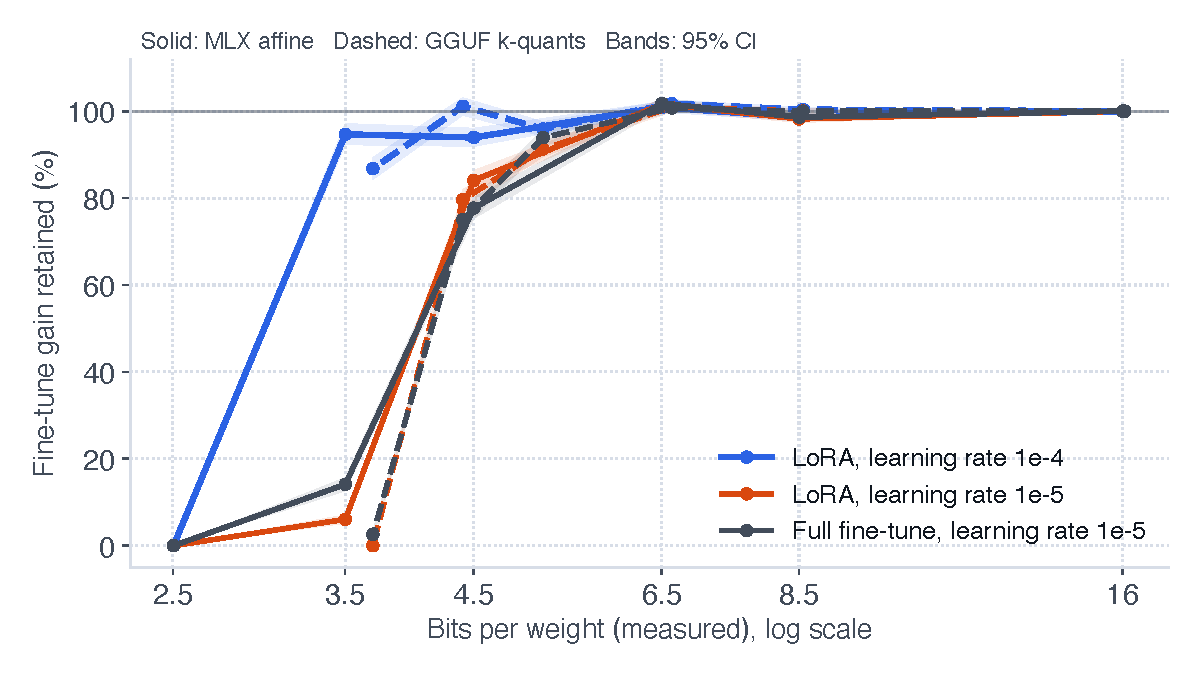
\includegraphics[width=0.84\linewidth]{figures/retention-q06.pdf}
\caption{Gain retained by three Qwen3-0.6B fine-tunes on banking77 against measured bits per weight (log scale; 16 is bf16): the LoRA at $10^{-4}$ (blue), the LoRA at $10^{-5}$ (orange) and full fine-tuning at $10^{-5}$ (dark gray). Solid lines: MLX affine; dashed: GGUF k-quants; bands: 95\% bootstrap intervals. The strong LoRA holds down to MLX~3-bit; the other two collapse there. Round 1, exploratory.}
\label{fig:retention}
\end{figure}

\subsection{Round 2: the smaller the update, the larger the loss}
\label{sec:lr}

Round 2 swept the learning rate on Qwen3-0.6B (Table~\ref{tab:lrsweep}, Figure~\ref{fig:lrsweep}). Learning rate is the variable we manipulated; within each kind of fine-tuning, the update norm $\lVert\Delta\rVert$ grows with it. Gain retention was positively rank-correlated with learning rate in all eight combinations of fine-tuning kind and format we tracked at 3 and 4 bits: Spearman $\rho = 1.0$ in seven, and $0.8$ for LoRA at Q4\_K\_M, where $3\times10^{-5}$ and $10^{-4}$ are tied to within 0.001. Each combination has only three or four learning rates, so each is weak evidence alone. The bf16 accuracies did not rank the same way: the most accurate model at full precision, the LoRA at $10^{-5}$, kept 6\% of its gain at MLX~3-bit. A second seed reproduced retention closely (LoRA at $10^{-4}$: 0.95 and 0.92 at MLX~3-bit; at $10^{-5}$: 0.06 and 0.00), while bf16 accuracy moved more (73.5\% and 65.1\% for the LoRA at $10^{-4}$). On Qwen3-1.7B, the LoRA at $10^{-5}$ kept 36\% of its gain at MLX~3-bit and the LoRA at $10^{-4}$ kept 163\%. In accuracy retention, which the collapsing base does not inflate, the pair is 0.32 against 0.93.

\begin{table}[htbp]
\centering\small
\caption{Gain retention $R$ by learning rate, Qwen3-0.6B on banking77, seed 0 (round~2, exploratory). $\lVert\Delta\rVert$ is the norm of the update over all fine-tuned linear layers. The LoRA at $3\times10^{-4}$ failed to learn and is omitted.}
\label{tab:lrsweep}
\begin{tabular}{llrrrrrrr}
\toprule
Kind & Learning rate & $\lVert\Delta\rVert$ & bf16 accuracy & MLX~4-bit & MLX~3-bit & Q4\_K\_M & Q3\_K\_M & Q2\_K \\
\midrule
\tablerows{tables/lrsweep.tex}
\bottomrule
\end{tabular}
\end{table}

\begin{figure}[htbp]
\centering
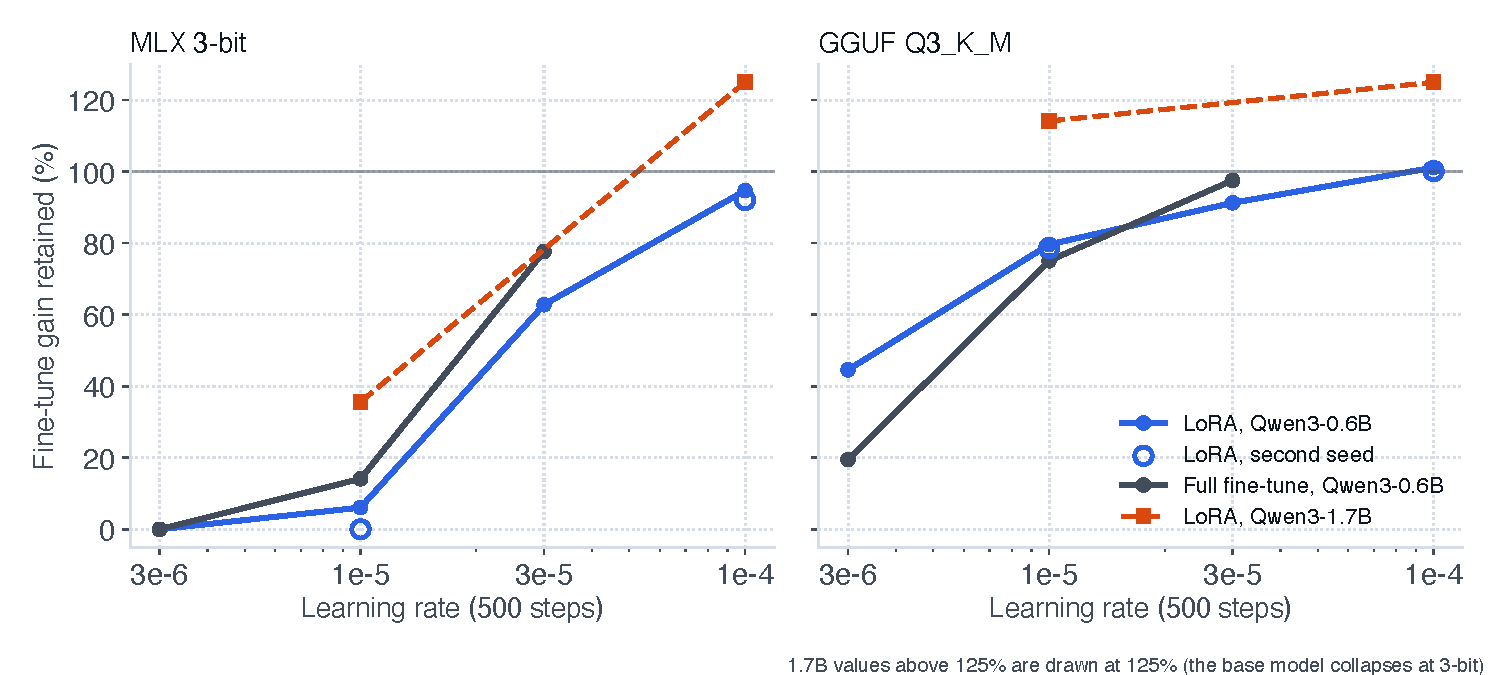
\includegraphics[width=\linewidth]{figures/lr-sweep.pdf}
\caption{Gain retained at MLX~3-bit and GGUF~Q3\_K\_M against learning rate. Qwen3-1.7B values above 125\% are drawn at 125\%, because its base collapses at 3 bits. Round 2, exploratory.}
\label{fig:lrsweep}
\end{figure}

\subsection{Why small updates break}
\label{sec:mech-results}

Figure~\ref{fig:mechanism} plots gain retention against NSR for the round-1 Qwen3-0.6B fine-tunes. Retention stays above 90\% while the rounding noise is up to about three times the update, and falls when it is larger. Table~\ref{tab:bands} makes this concrete over all 89 fine-tune and format pairs from rounds 1 and 2. When the base is intact and most of the update survives, all 44 pairs with NSR below 3 kept at least 90\% of their gain, against 3 of 7 between 3 and 5 and 4 of 10 at 5 or more. The bands were chosen after looking at these data, so the table describes them and tests nothing.

\begin{figure}[htbp]
\centering
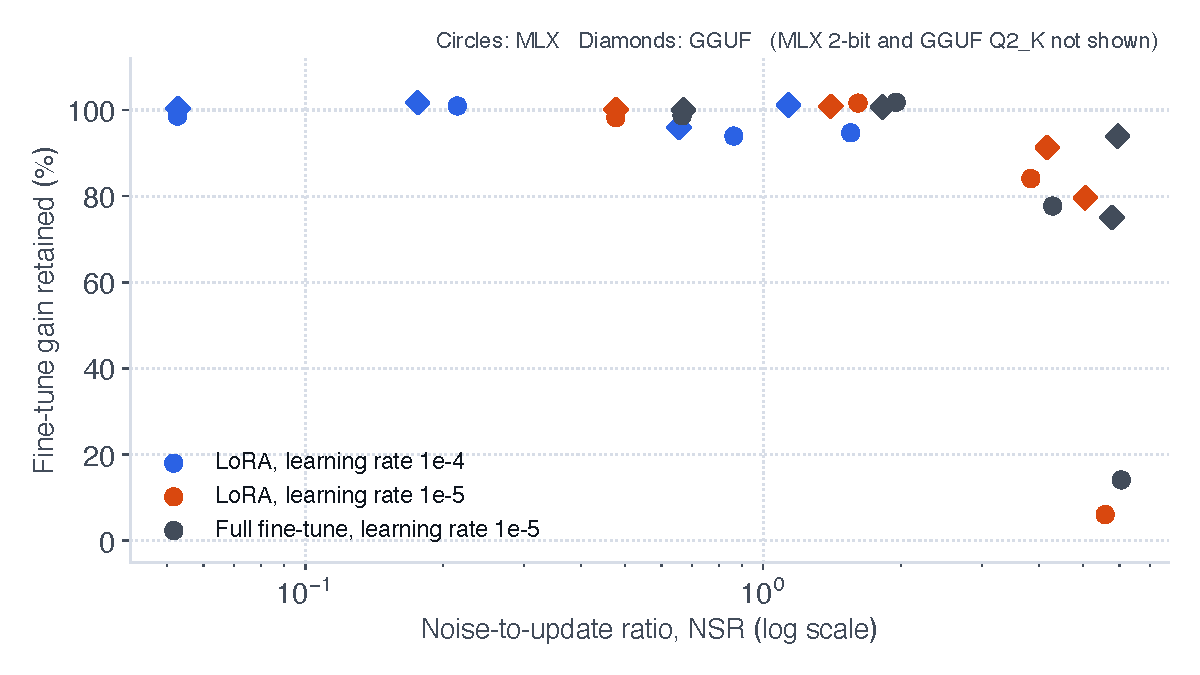
\includegraphics[width=0.84\linewidth]{figures/mechanism-q06.pdf}
\caption{Gain retained against the noise-to-update ratio NSR (log scale) for the round-1 Qwen3-0.6B fine-tunes, at every format except MLX~2-bit and GGUF~Q2\_K. The base model also breaks at MLX~3-bit; the two points at the lower right are the gentle LoRA and the full fine-tune there. Circles: MLX; diamonds: GGUF.}
\label{fig:mechanism}
\end{figure}

\begin{table}[htbp]
\centering\small
\caption{Gain retention by measurement band, over the 89 fine-tune and format pairs of rounds 1 and 2 (Qwen3-0.6B and Qwen3-1.7B on banking77). The bands were chosen after seeing these data.}
\label{tab:bands}
\begin{tabular}{lrrr}
\toprule
Measurement & Pairs & Kept $\ge 90\%$ of gain & Lowest \\
\midrule
base damage $< 1$, update kept $\ge 60\%$, NSR $< 3$ & 44 & 44 & 91\% \\
base damage $< 1$, update kept $\ge 60\%$, NSR 3 to 5 & 7 & 3 & 78\% \\
base damage $< 1$, update kept $\ge 60\%$, NSR $\ge 5$ & 10 & 4 & 45\% \\
update kept $< 60\%$ & 4 & 0 & 0\% \\
update kept $\ge 60\%$, base damage $\ge 1$ & 24 & 4 & 0\% \\
\bottomrule
\end{tabular}
\end{table}

The fourth row is the second failure mode. Full fine-tuning at $3\times10^{-6}$ produces an update so small, relative to the 3-bit quantization step, that the fine-tuned and base weights round to the same codes: only 5.5\% of its update's projection survives MLX~3-bit. Little noise is added because almost nothing is left, so its NSR (2.16) looks benign, and its measured gain retention is 0\%. At MLX~4-bit the same fine-tune keeps 50\% of its update and 27\% of its gain. Across all four rounds this was rare: of 192 measured pairs, the five that kept less than 60\% of their update were all full fine-tunes, four of them from the run at $3\times10^{-6}$.

The last row is a second axis. When the base model itself breaks, with base damage of 1 or more (for Qwen3-0.6B and Qwen3-1.7B: MLX~3-bit and 2-bit and GGUF~Q2\_K), only large updates held on: 4 of 24 such pairs kept 90\% of their gain. A large update can carry a broken base: at MLX~3-bit the Qwen3-0.6B base scored 0\%, while its LoRA at $10^{-4}$ kept 95\% of its gain. The noise ratio does not separate every case. At Q2\_K, full fine-tuning at $3\times10^{-5}$ kept 89\% of its gain while LoRA at $3\times10^{-5}$ kept 1\%, with almost the same NSR (5.29 and 5.16) on the same base. One untested explanation is that full fine-tuning also changes the RMSNorm weights, which neither format quantizes.

\subsection{Rounds 3 and 4: replication across family, task, seed and size}
\label{sec:replication}

Rounds 3 and 4 turned the round-2 observation into confirmatory tests. Each test asks whether the LoRA at $10^{-4}$ keeps more of its gain than the LoRA at $10^{-5}$, by a paired bootstrap of $R(10^{-4}) - R(10^{-5})$, at MLX~3-bit and at Q3\_K\_M. A test is supported only if its 95\% interval lies above zero. Round 3 moved to a new model family (OLMo-2 1B on banking77) and a new task (Qwen3-0.6B on MASSIVE); round~4 repeated both with a second seed and added Qwen3-4B. All 10 tests were supported (Table~\ref{tab:replication}). The differences ranged from $+0.06$ (OLMo at Q3\_K\_M, with both seeds) to $+0.63$ (MASSIVE at MLX~3-bit, seed 1). Values of $R$ above 1 again reflect a base that loses more than the fine-tune: the OLMo base falls from 14.5\% to 6.8\% at MLX~3-bit, and the 4B base from 57.5\% to 42.9\%.

\begin{table}[htbp]
\centering\footnotesize
\caption{The ten pre-registered tests of whether the LoRA at $10^{-4}$ keeps more of its gain than the LoRA at $10^{-5}$. Difference is $R(10^{-4}) - R(10^{-5})$ with a 95\% paired bootstrap interval.}
\label{tab:replication}
\begin{tabular}{lllcrrll}
\toprule
Test & Setting & Seed & Format & $R$, $10^{-4}$ & $R$, $10^{-5}$ & Difference [95\% CI] & Verdict \\
\midrule
\tablerows{tables/replication.tex}
\bottomrule
\end{tabular}
\end{table}

Table~\ref{tab:pattern} and Figure~\ref{fig:replication} show accuracy retention for every setting in which both LoRAs were trained, including the two Qwen3 banking77 settings from rounds 1 and 2. In all seven, the gentle LoRA had the higher bf16 accuracy and kept less of its accuracy at each of the five formats compared (MLX~4-bit and 3-bit, GGUF~Q4\_K\_M, Q3\_K\_M and Q2\_K): 35 comparisons in the same direction. MLX~2-bit, evaluated only in round~1, left both Qwen3-0.6B LoRAs at 0\%. Two cautions apply. The seven settings are not independent, since two are second seeds of others. And at Q4\_K\_M the gaps are small: five of the seven are under 2 points, and one is 0.3 points. At 3 bits and below, every gap is at least 4.5 points.

\begin{figure}[htbp]
\centering
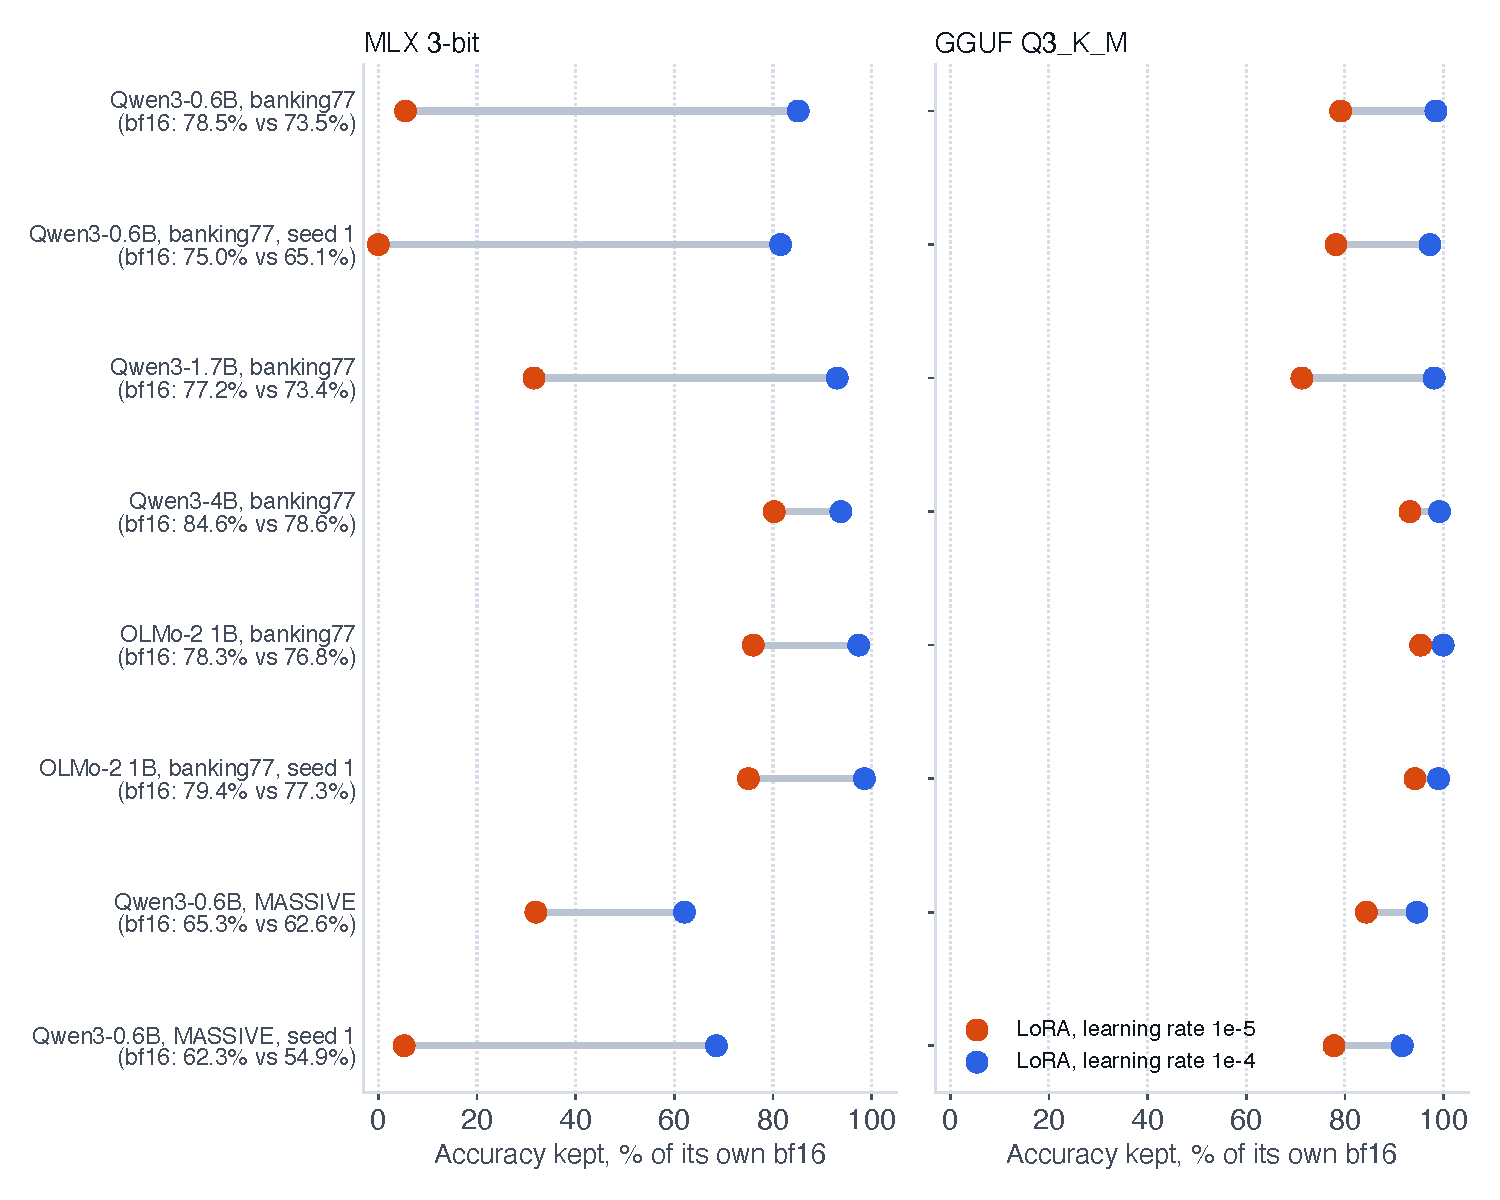
\includegraphics[width=\linewidth]{figures/replication.pdf}
\caption{Accuracy kept, as a share of each model's own bf16 accuracy, by the LoRA at $10^{-5}$ (orange) and the LoRA at $10^{-4}$ (blue), at MLX~3-bit and GGUF~Q3\_K\_M, in all seven settings. Labels give the two bf16 accuracies.}
\label{fig:replication}
\end{figure}

\begin{table}[htbp]
\centering\footnotesize
\caption{Accuracy retention $A$ at the five formats compared. Each cell gives the gentle LoRA ($10^{-5}$) / the strong LoRA ($10^{-4}$); the first column gives their bf16 accuracies in percent. Exploratory. $^\dagger$Gap under 0.01 (0.003).}
\label{tab:pattern}
\begin{tabular}{lcccccc}
\toprule
Setting & bf16 accuracy & MLX~4-bit & MLX~3-bit & Q4\_K\_M & Q3\_K\_M & Q2\_K \\
\midrule
\tablerows{tables/pattern.tex}
\bottomrule
\end{tabular}
\end{table}


Qwen3-4B differs in degree. Its base does not break at MLX~3-bit by the tool's rule (base damage 0.64, against 1.21 for Qwen3-0.6B and 1.08 for 1.7B) and keeps 74\% of its accuracy there. The gap between its two LoRAs is smaller than for Qwen3-0.6B or Qwen3-1.7B at MLX~3-bit, Q3\_K\_M and Q2\_K, most of all at MLX~3-bit (0.80 against 0.94, compared with 0.06 against 0.85 at 0.6B). At Q2\_K, where the 4B base does break (15.8\% accuracy, base damage 1.03), its gentle LoRA still loses 40\% of its accuracy. With one fine-tune pair per size, and learning rates that were not rescaled for size, these numbers do not establish a trend with size.

Across seeds, OLMo reproduced closely: at MLX~3-bit and Q3\_K\_M, $R$ moved by at most 0.02 and bf16 accuracy by 1.1 points; at other formats $R$ moved by up to 0.04. MASSIVE did not. The direction held, but the gentle LoRA's gain retention at MLX~3-bit went from 0.32 with seed 0 to 0.05 with seed 1, and the strong LoRA's bf16 accuracy fell 7.7 points.

\subsection{Predicting retention before quantizing}
\label{sec:predictor}

Round 2 tested whether the weight measurements predict gain retention. Predictor v1 was fitted by least squares against $R$ clipped to $[0,1]$, on the round-1 Qwen3-0.6B points only, and frozen:
\begin{equation}
\hat R = \sigma\left(8.707 - 5.81 \ln \mathrm{NSR} - 2.794 \ln \mathrm{KLD}_{\mathrm{base}}\right).
\end{equation}
Its test had three pre-registered criteria. On new learning rates and seeds, its mean absolute error (MAE) had to be at most 0.10, and its agreement with the measurements on the call ``keeps at least 90\%'' at least 0.85 (P1). It had to beat two baselines: the mean retention of each format (bits-only) and a one-feature model of base damage (KLD-only) (P2). On Qwen3-1.7B, its MAE had to be at most 0.15 and its agreement at least 0.80 (P3). P2 and P3 were met. P1 was not, by 0.007 (Table~\ref{tab:predictor}), and as pre-registered, the tool was limited to descriptive output.

\begin{table}[htbp]
\centering\footnotesize
\caption{Pre-registered predictor tests. MAE is against $R$ clipped to $[0,1]$, with 95\% intervals from resampling whole fine-tunes. Safe is the share of points where predicted and measured retention fall on the same side of 0.9. W3-H2 and W4-H3 are the accuracy bars; W3-H3 and W4-H4 require beating both baselines. $^\ast$Exploratory breakdown of 2 fine-tunes, without an interval.}
\label{tab:predictor}
\begin{tabularx}{\linewidth}{Lrlcccl}
\toprule
Test & $n$ & MAE [95\% CI] & Safe & KLD-only & Bits-only & Result \\
\midrule
\tablerows{tables/predictor.tex}
\bottomrule
\end{tabularx}
\end{table}

The largest miss explained the failure. Predictor v1 predicted 98\% retention for the full fine-tune at $3\times10^{-6}$ at MLX~3-bit, whose update is rounded away. NSR measures only the noise, so it read a vanished update as safe. Predictor v2 adds update kept:
\begin{equation}
\hat R = \sigma\left(5.612 + 3.296 \ln \frac{\mathrm{kept}}{\mathrm{NSR}} - 1.555 \ln \mathrm{KLD}_{\mathrm{base}}\right).
\end{equation}
Its form was chosen among four candidates by cross-validation that leaves out one fine-tune at a time, on all 89 round-1 and round-2 points (error 0.071, against 0.095 for the v1 form), and it was fitted on those points and frozen before round~3.

Predictor v2 passed both of its pre-registered tests (Table~\ref{tab:predictor}, Figure~\ref{fig:predictor}): an accuracy bar, MAE at most 0.10 with safe-call agreement at least 0.85 (W3-H2, W4-H3), and a lower MAE than both baselines (W3-H3, W4-H4). On round~3 (OLMo-2 1B and MASSIVE, 35 points) its MAE was 0.059, with safe-call agreement 0.94, below both baselines. On round~4 (second seeds and Qwen3-4B, 42 points) it was 0.084 with agreement 0.90, again below both baselines, but by a thinner margin. The interval reaches 0.146, above the 0.10 bar, and overlaps the KLD-only interval. Predictor v1 did almost as well (0.090), and better on the MASSIVE arm (0.072 against 0.088); it would also have met the accuracy bar in both rounds (0.071 and 0.090). No held-out fine-tune entered the rounded-away regime (the lowest update kept was 74\% in round~3 and 98.5\% in round~4), so the benefit of adding update kept has not been tested out of sample. Without the easy 6-bit formats, v2's round-4 error was 0.115, against 0.080 in round~3.

\begin{figure}[htbp]
\centering
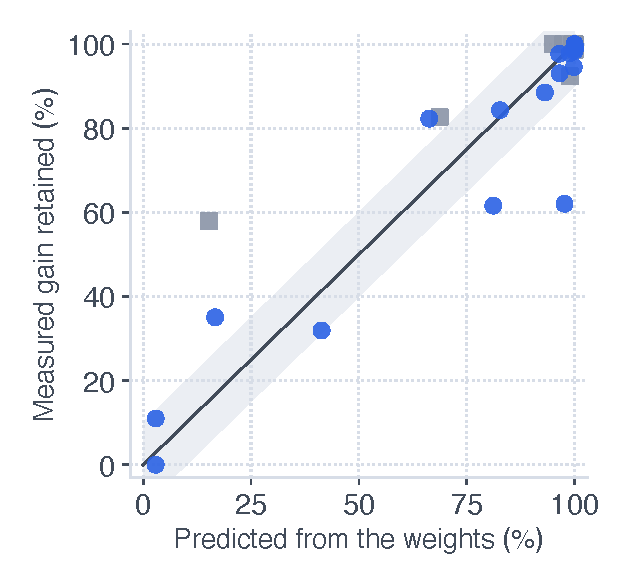
\includegraphics[width=0.49\linewidth]{figures/predictor-v2-week3.pdf}\hfill
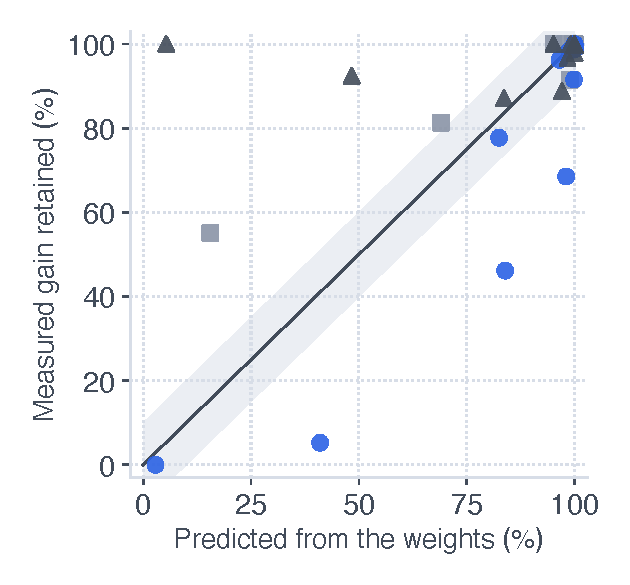
\includegraphics[width=0.49\linewidth]{figures/predictor-v2-week4.pdf}
\caption{Predictor v2's predictions, made from the weights without evaluating the quantized models, against measured gain retention (capped at 100\%). Left: round~3, 35 points (squares: OLMo-2 1B on banking77; circles: Qwen3-0.6B on MASSIVE). Right: round~4, 42 points (squares: OLMo-2 1B, seed 1; circles: Qwen3-0.6B on MASSIVE, seed 1; triangles: Qwen3-4B on banking77). The band marks $\pm 10$ points.}
\label{fig:predictor}
\end{figure}

The misses follow two patterns. On MASSIVE, when the base breaks, the slot-annotation task loses more than a small noise ratio suggests: the LoRA at $10^{-4}$ at MLX~3-bit was predicted to keep 98\% of its gain and kept 62\% (seed 0) and 69\% (seed 1). On banking77, the OLMo and Qwen3-4B fine-tunes kept more than a large noise ratio suggests: the gentle 4B LoRA kept 92\% of its gain at MLX~3-bit with NSR 6.85, where v2 predicted 48\%. At Q2\_K the same model has $R = 1.28$ against a prediction of 5\%, but only because its base collapsed; the fine-tune itself kept 60\% of its accuracy. On the 14 Qwen3-4B points alone, v2's MAE was 0.115 and its agreement 0.79, short of both bars. That breakdown was not pre-registered. After seeing it, we decided that \texttt{ftquant check} would not predict for Qwen3-4B.

\subsection{Operating points drift before accuracy}
\label{sec:drift}

This section is exploratory. The one pre-registered test of operating-point drift, round-1 H4 at 4 bits, was not supported, because GGUF~Q4\_K\_M moved coverage by only 1.2 points. At lower bit widths the picture changes. For the round-1 Qwen3-1.7B LoRA, MLX~3-bit kept 93\% of the accuracy but cut the share of auto-accepted items from 38.1\% to 27.8\%, and Q2\_K kept 85\% of the accuracy but cut coverage from 36.4\% to 10.1\%. In the examples we examined, the gentle fine-tunes drifted more. At MLX~4-bit, the Qwen3-0.6B LoRA at $10^{-5}$ kept 88.5\% of its accuracy but accepted 19.4 points fewer items. The OLMo LoRA at $10^{-5}$ kept 76\% of its accuracy at MLX~3-bit and accepted 33.5 points fewer, and the gentle Qwen3-4B LoRA kept 60\% at Q2\_K and accepted 67.9 points fewer. A system that sends low-confidence outputs to a person would see that workload change at formats where accuracy still looks acceptable. This is a single-threshold counterpart of what \citet{zhu2026conformal} report for conformal prediction under configuration shift.

\section{The \texttt{ftquant check} tool}
\label{sec:tool}

\texttt{ftquant check} implements Section~\ref{sec:mechanism} for a user's own fine-tune. It reads an MLX or PEFT adapter, or a full checkpoint, streams the safetensors, and runs the exact quantizer on the base and fine-tuned weights. It prints update kept, NSR and base damage. It adds v2's prediction only where v2 was tested: MLX 6, 4 and 3-bit with group size 64 and GGUF~Q6\_K, Q4\_K\_M, Q3\_K\_M and Q2\_K, on the three bases whose base damage ships with the tool (Qwen3-0.6B, Qwen3-1.7B and OLMo-2 1B). v2 was fitted on Qwen3-0.6B and Qwen3-1.7B banking77 fine-tunes and tested on held-out OLMo-2 1B, Qwen3-0.6B MASSIVE and Qwen3-4B fine-tunes. The tool needs only numpy. For a Qwen3-0.6B LoRA trained on MASSIVE at $10^{-5}$, a fine-tune v2 had never seen, it printed:

\begin{scriptsize}
\begin{verbatim}
format                     noise/update  update kept  base damage  predicted gain kept  reading
MLX 8-bit (group 64)               0.47         100%        0.004                  n/a  low noise
MLX 6-bit (group 64)               1.59         100%        0.021                 100%  low noise
MLX 4-bit (group 64)               3.80         100%        0.255                  97%  moderate noise
MLX 3-bit (group 64)               5.52          99%        1.207                  41%  high noise, base model breaks
\end{verbatim}
\end{scriptsize}

\noindent Measured on its 2,974 test items, that fine-tune kept 93\% of its gain at MLX~4-bit and 32\% at 3-bit. The reading column uses the bands of Table~\ref{tab:bands}. The seed-1 run of the same configuration had almost identical measurements and the same 41\% prediction at MLX~3-bit, but kept 5\% of its gain: weight measurements cannot see seed-to-seed variation of this size.

\section{Limitations}
\label{sec:limits}

\begin{itemize}
\item \textbf{Scale.} Four base models, none larger than 4B. Only Qwen3-4B is above 1.7B, and it was run with one seed on one task, with gradient accumulation where the other runs had none.
\item \textbf{Tasks.} Two tasks, both with short outputs and scored by exact match, so format failures count as errors. Much of the bases' collapse at 3 bits is a loss of valid outputs, which inflates $R$. Long-form generation may degrade differently.
\item \textbf{Fine-tuning.} LoRA rank 8 only, 500 steps, and the same nominal learning rates at every size, so ``gentle'' may not mean the same update size at 4B. The 4B base already scores 57.5\% zero-shot, so its fine-tunes' gains (21 and 27 points) are smaller than elsewhere and their $R$ values noisier. Full fine-tuning was run only on Qwen3-0.6B, and only in exploratory analyses.
\item \textbf{Formats.} MLX group size 64 only, GGUF without an importance matrix, and no calibration-based methods such as GPTQ or AWQ.
\item \textbf{Metric.} $R$ exceeds 1 whenever the base loses more than the fine-tune, which makes it hard to read at 3 bits and below. We report accuracy retention next to it.
\item \textbf{Uncertainty.} Bootstrap intervals cover test-set sampling only; seed-to-seed variation can be larger (Section~\ref{sec:replication}).
\item \textbf{Predictor.} Its round-4 interval crosses the 0.10 bar, and it fails on the 4B subgroup. Its added input, update kept, targets a failure mode that no held-out fine-tune reached. Its reading bands were chosen post hoc.
\item \textbf{Operating point.} $\tau$ was fitted on half of the test set rather than the planned validation split.
\item \textbf{Process.} One researcher and one machine, with no external review of the pre-registrations before the runs.
\end{itemize}

\section{Conclusion}
\label{sec:conclusion}

In pre-registered tests on three base models, two tasks, and a second seed for two of them, the gentle LoRA kept less of its gain at 3 bits than the strong LoRA, and exploratory comparisons at 4 bits point the same way with smaller margins. The weight-space picture is consistent with this: quantization keeps an update's projection and adds noise, so small updates drown or round away. Two practical consequences follow. A fine-tune should be selected on the quantized artifact it will ship as, not on its bf16 score. And when training is cheap, a larger update may buy robustness at a small cost in bf16 accuracy; our data show this trade, not where its optimum lies. A check that needs only the weights and a one-time measurement of the base model can flag risky formats before any task evaluation, as long as its predictions are trusted only where they have been tested.

\phantomsection\addcontentsline{toc}{section}{References}
\bibliographystyle{plainnat}
\bibliography{refs}

\appendix

\section{Deviations from the pre-registered plans}
\label{app:deviations}

\begin{table}[h]
\centering\footnotesize
\begin{tabularx}{\linewidth}{llLL}
\toprule
When (PDT) & Round & Deviation & Effect \\
\midrule
27 Sep, 18:00 & 1 & The analysis code for $\tau$ was changed to match the written definition, before any 1.7B result existed. & None on confirmatory results. \\
27 Sep, 23:48 & 2 & The predictor freeze step crashed on a missing folder before writing anything, and was re-run. & None. \\
28 Sep, 08:29 & 2 & LoRA at $3\times10^{-4}$ failed to learn, so its $R$ is undefined; its 7 points were excluded from the round-2 test on new learning rates and seeds (P1, P2). & That test was scored on 42 points instead of 49 (Table~\ref{tab:predictor}). \\
29 Sep, 05:16 & 4 & The 4B fine-tunes ran out of memory at batch size 4 and were trained with micro-batches of 2 and two-step accumulation. & Same effective batch, steps and examples. \\
29 Sep, 16:29 & 2 to 4 & $\tau$ was fitted on half of the test set, not the validation split the round-1 plan named for later rounds. Found in an audit. & Exploratory drift numbers only. \\
\bottomrule
\end{tabularx}
\end{table}

\section{Reproducibility and compute}
\label{app:repro}

Software: MLX 0.32.2 and mlx-lm 0.31.3; llama.cpp build 11146 (commit 7fe450e19), whose \texttt{gguf-py} and converter are vendored at the same commit. Data: PolyAI's banking77 CSV files and Amazon's MASSIVE release, both checked against recorded SHA-256 hashes by the fetch script. The repository holds the four pre-registrations and their hash logs, the frozen predictors (v1 SHA-256 prefix \texttt{5df7d620}, v2 \texttt{6fd78627}), the per-item predictions of every evaluation, every training configuration and log, and a lab notebook written as the runs happened. At the time of writing the repository is private.

Everything ran on one Apple M1 Pro laptop with 16 GB of memory, in about 51 hours of wall-clock time from the first sweep (27 September, 12:45) to the last verdicts (29 September, 16:12). A LoRA run of 500 steps took 10 to 20 minutes on Qwen3-0.6B, 52 to 56 minutes on 1.7B, 40 to 53 minutes on OLMo-2 1B and 2 hours 8 minutes to 2 hours 24 minutes on 4B. One full-test-set evaluation took 2 to 23 minutes on the smaller models and 12 to 25 minutes on 4B. The mechanism measurements for two fine-tunes took 5 to 8 minutes on the 0.6B and 1B models and 30 minutes on 4B.

\end{document}
